\chapter{\label{chapter4}Implementation}

In this chapter, we show how we integrated Swift into iSDX. We give an overview of the modified iSDX architecture in \ref{chapter4:Architecture}. We explain the two new modules that were added to the iSDX in \ref{chapter4:Swift-BPA} and  \ref{chapter4:FR-handler}. Then, we show how we combined the VMAC schemes of Swift and iSDX and partitioned the available bits among the two in \ref{chapter4:vmac_partitioning}. At last, we explain how the default iSDX modules had to be adapted in \ref{chapter4:Changes_to_the_iSDX}.

In the next chapter, we present the results of the tests done to measure the convergence performance of the iSDX.

\section{\label{chapter4:Architecture}Architecture}

\begin{figure}[h]
\center
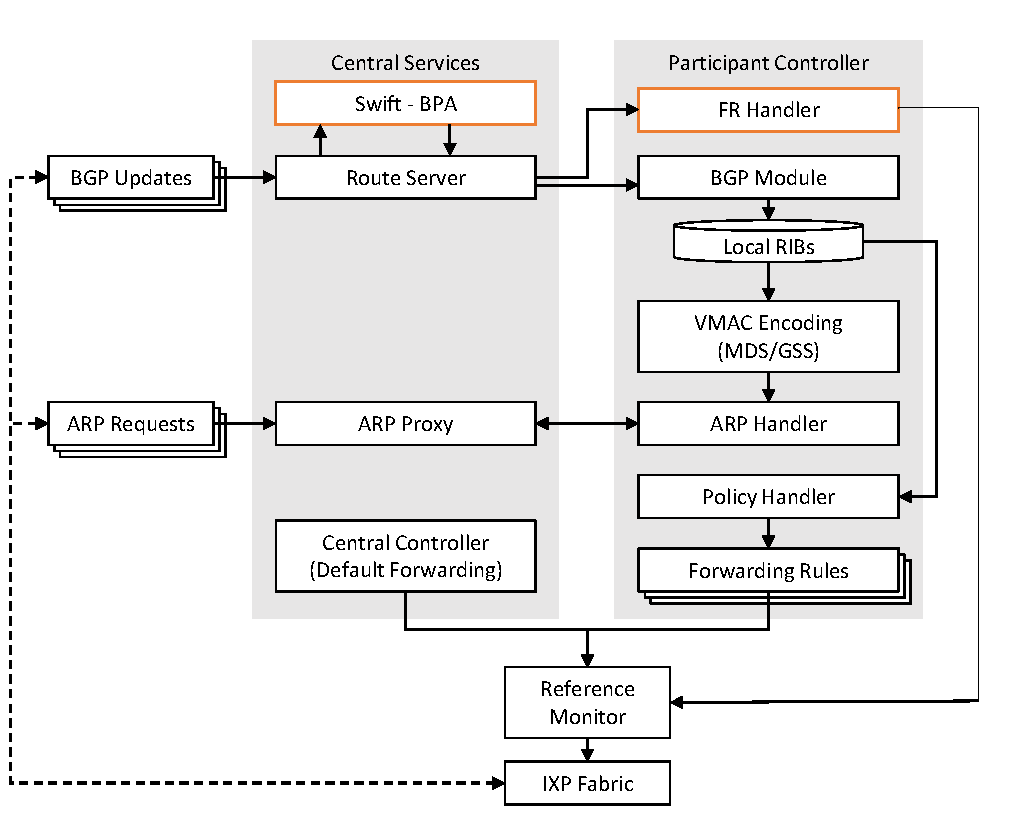
\includegraphics[scale = 0.5]{Figures/design_sdx_swift_cropped.pdf}
\caption{iSDX architecture with Swift}
\label{fig:isdx_architecture_with_swift}
\end{figure}

Figure~\ref{fig:isdx_architecture_with_swift} shows the iSDX~\cite{feamster2013sdx} architecture with Swift. The orange modules represent the new modules we had to add to the iSDX to implement Swift. The iSDX receives two additional modules the Swift-BPA module in the central services and the FR handler in the participant controller. With these two modules the iSDX is able to detect bursts of withdrawals, predict the failed AS-link that caused the burst and push fast reroute rules into the IXP fabric.

In the following sections, we explain the functionality of the new modules and other changes to the iSDX in more detail.

\section{\label{chapter4:Swift-BPA}Swift-BPA}

\begin{figure}[h]
\center
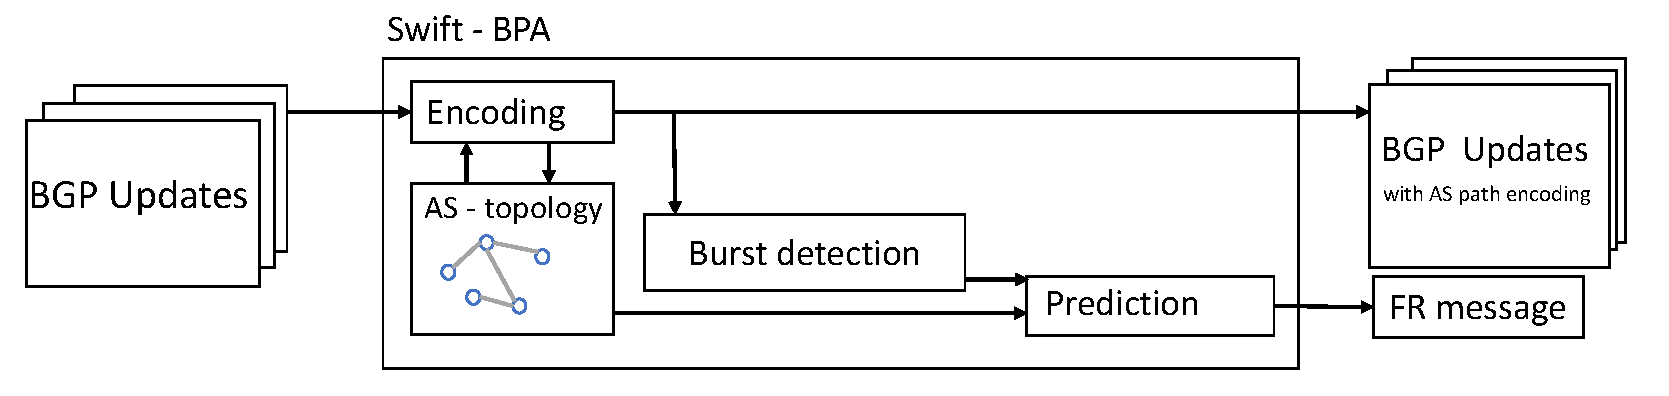
\includegraphics[scale = 0.5]{Figures/design_swift_bpa_cropped.pdf}
\caption{pipeline of the Swift-BPA module}
\end{figure}

The Swift-BPA module implements Swifts main functionality, encoding and prediction. It is part of the central services and exchanges BGP updates and fast reroute (FR) messages with the route server and participant controllers.

The Swift-BPA module is placed in the route server and processes each update received by the route server before passing it on to the participant controllers. 
Similar to the participant controller every participant has a Swift-BPA process running. The Swift-BPA only receives BGP updates from his own routers. This way the Swift engine can be implemented without any modifications.

When receiving a BGP update the Swift-BPA updates the AS-topology and adds the AS-path encoding to the BGP update. The AS-topology is used when predicting a failed AS-link, it stores AS-links and the number of received routes that traverse this link. Then the update gets sent to the participant controller. The AS-path encoding is used in the Swift part of the VMAC. 
After the update is sent to the participant controller the burst detection checks if the update triggers a burst. If so the prediction module predicts the failed AS-link, the cause of the burst and sends FR messages to the participant controllers. 
The FR messages inform the participant controllers about the AS-link that is predicted to be down. In the following, we show how the participant controllers handle the FR messages.


\section{\label{chapter4:FR-handler}FR Handler}

\begin{figure}[h]
\center
\includegraphics[scale = 0.6]{Figures/design_fr_handler_cropped.pdf}
\caption{pipeline of the fast reroute handler}
\end{figure}

The FR-handler is placed in the participant controller and processes FR messages.
Upon receiving a FR message the FR handler computes the FR rules. The FR rules are computed using the failed AS-link contained in the FR message and the backup next-hops, which were computed by the participant controller. 
The FR rules get sent to the reference monitor as flow rule messages. The reference monitor then installs the flow rules in the SDN switch. Just like in Swift the FR rules match on the failed AS-link and on the backup next-hop.    

\newpage

\section{\label{chapter4:vmac_partitioning}VMAC Partitioning}

Both Swift and iSDX use the destination MAC address as a VMAC to attach additional information to the packet. It is not easy to use another field of the header as only the destination MAC address can be changed by modifying the next hop attribute. Therefore the VMAC has to be shared between the iSDX and the Swift encoding. The number of bits available to encode information for the iSDX and Swift is reduced. This is because the iSDX and Swift encode 
different information about the prefix. The iSDX encodes the participants advertising the prefix and the BGP best next hop. Swift encodes the AS-path and the backup next hops for each link on the AS-path.

The encoded AS-path starts with the second AS on the AS-path. This is because the first AS is already encoded as the BGP best next-hop. (in the iSDX part of the VMAC)

\begin{figure}[h]
\center
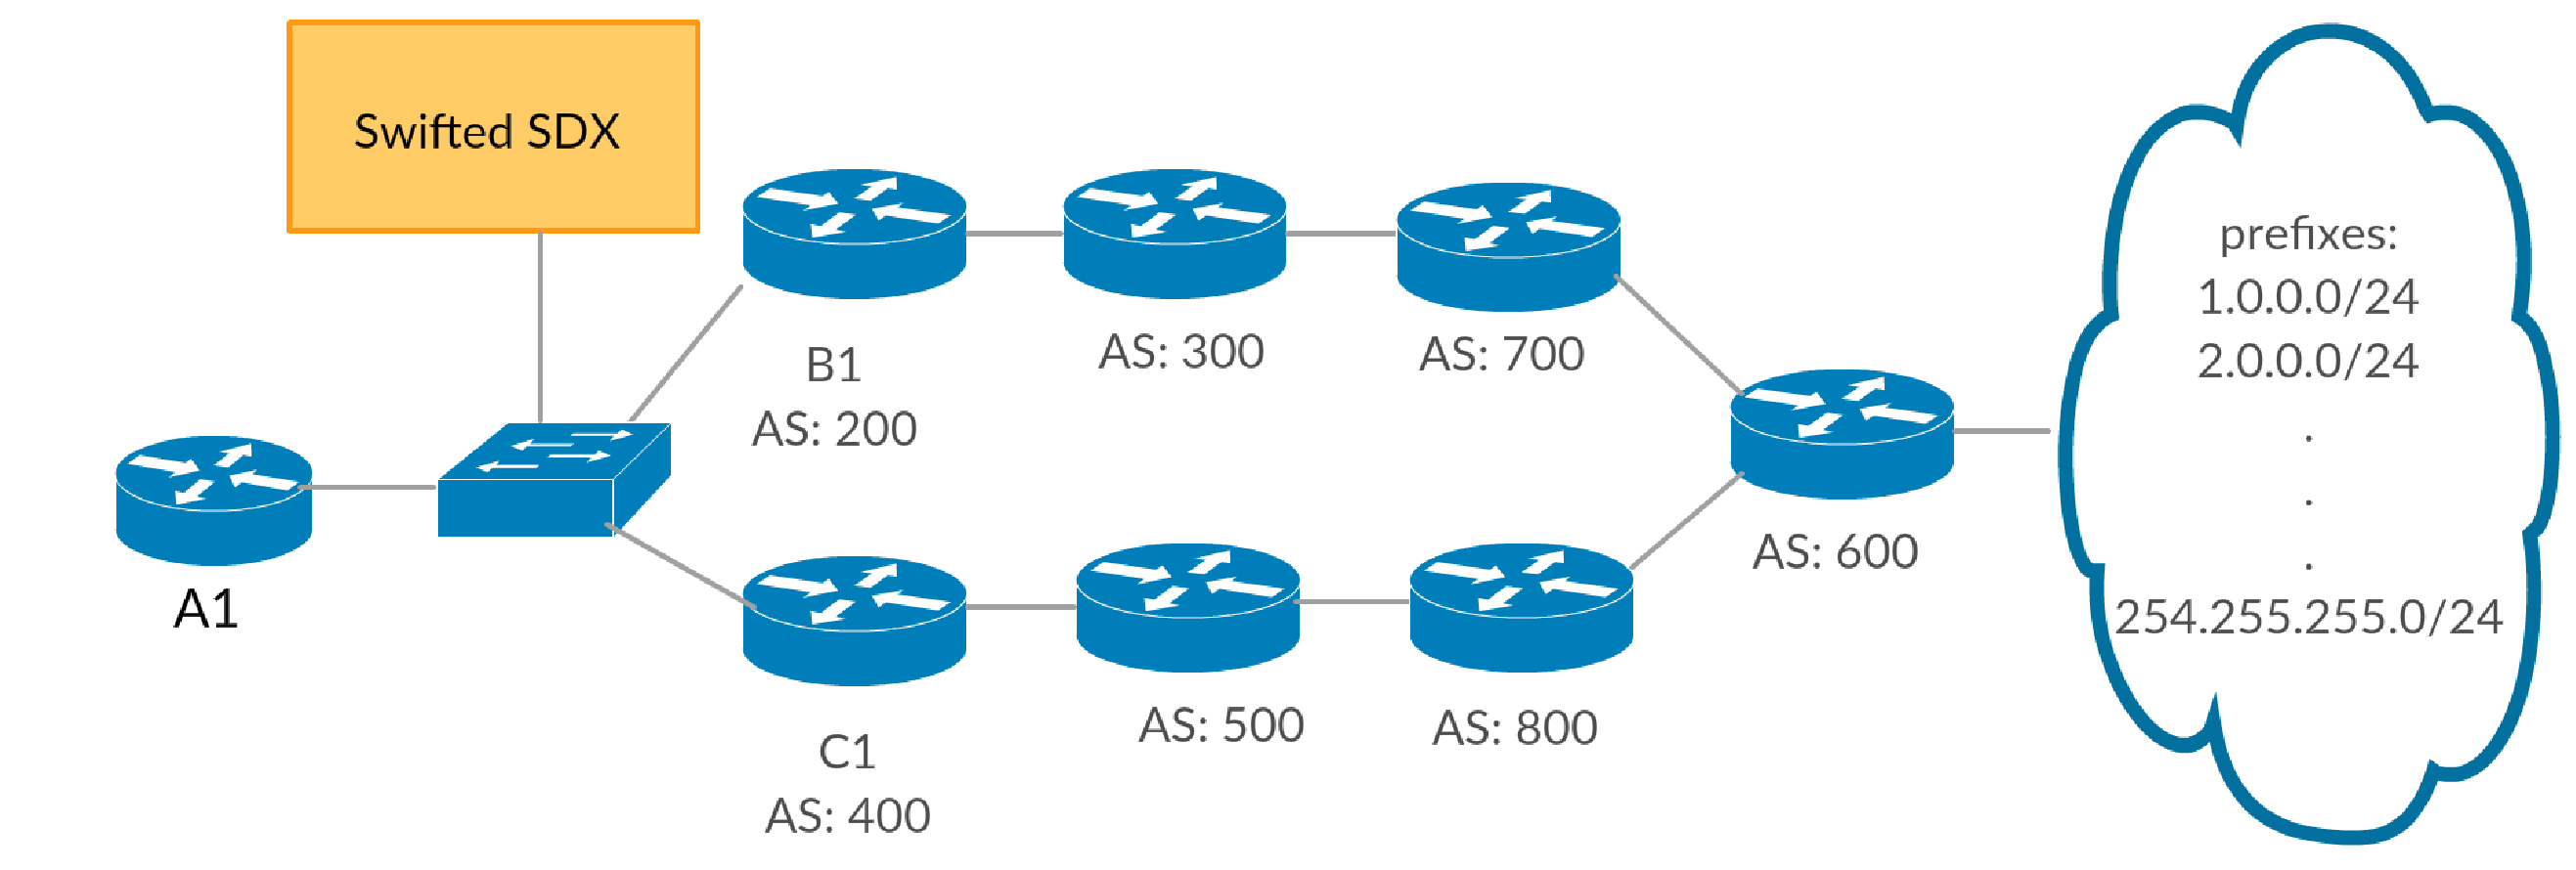
\includegraphics[scale = 0.24]{Figures/design_vmac_topology.pdf}
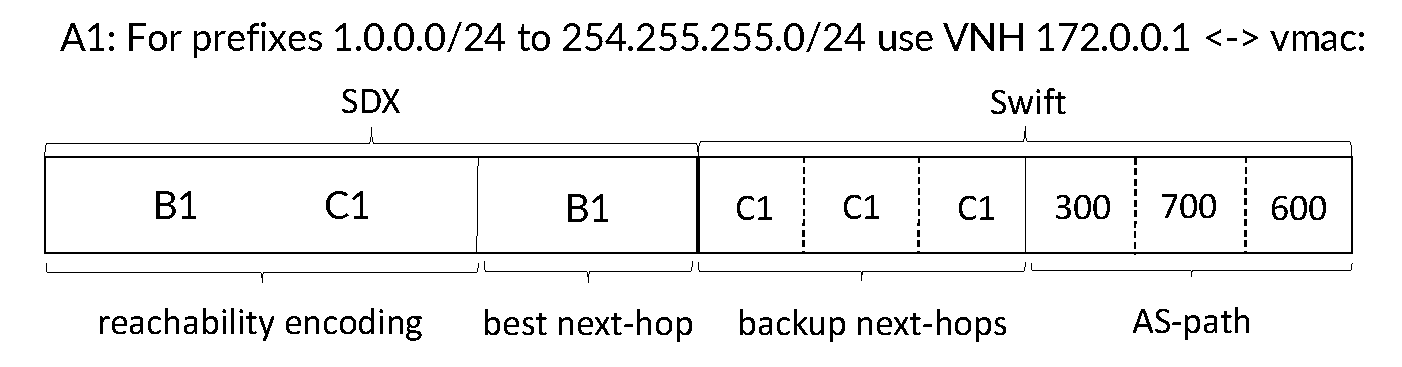
\includegraphics[scale = 0.35]{Figures/design_vmac_cropped.pdf}
\caption{example of the VMAC in the iSDX with Swift}
\end{figure}

\section{\label{chapter4:Changes_to_the_iSDX}Changes to the iSDX}

We had to apply a few changes to the iSDX's modules. These changes mainly affect the route server, the local RIB of the participant controller and the VMAC encoding. 

\paragraph{\label{chapter4:Changes to the iSDX:route server}Route Server:}

The route server had to be adapted to work with the Swift-BPA module. 
Instead of simply forwarding BGP updates from participant routers to the corresponding participant controller the route server forwards these updates to the corresponding Swift-BPA process. This is done so the Swift-BPA can augment the updates with the encoding of the AS-path. The route server also receives FR messages and augmented BGP updates with AS-path encoding from the Swift-BPA and forwards them to the corresponding participant controllers. 
\begin{figure}[h]
\center
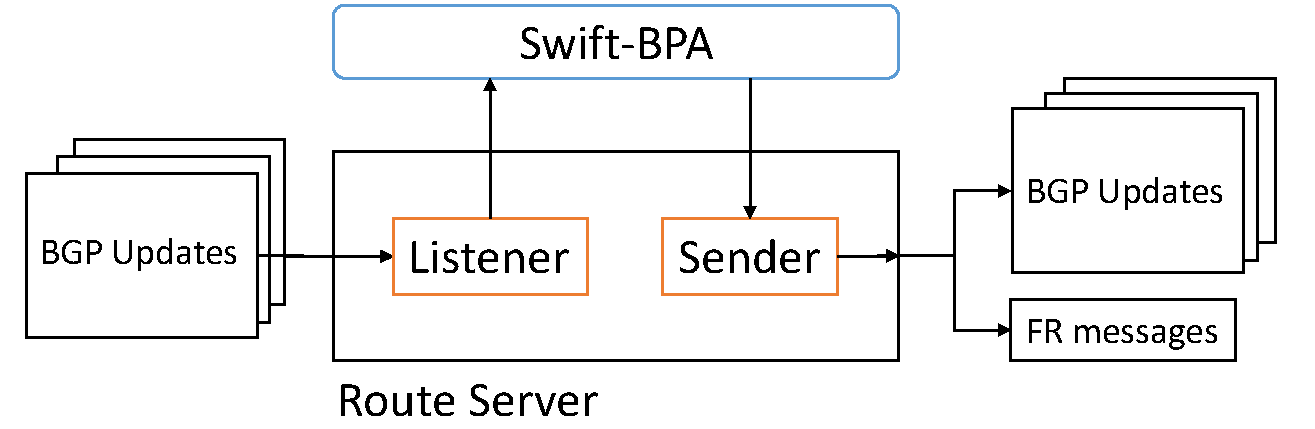
\includegraphics[scale = 0.45]{Figures/design_route_server_cropped2.pdf}
\caption{pipeline of the modified route server}
\end{figure}


\paragraph{\label{chapter4:Changes to the iSDX:local RIB}Local RIB:}

As each BGP update from the route server contains the AS-path encoding, the local RIB had to be adapted to store this information. 
When processing a BGP update the local RIB extracts the AS-path encoding (added by the Swift-BPA) and saves it as an additional attribute. The encoded AS-path is then used in the VMAC encoding. 

\paragraph{\label{chapter4:Changes to the iSDX:Vmac Encoding}VMAC Encoding:}
The VMAC encoding builds the VMAC with both  the iSDX and Swift information. The Swift encoding uses the AS-path encoding stored in the local RIB and the backup next-hops. The backup next-hops are computed by the VMAC encoding for the encoded AS-paths. There is one backup next-hop for every AS-link on the AS-path, packets can be sent to the backup next-hop in case this AS-link is predicted to be down. \\

\newpage
